\renewcommand{\baselinestretch}{2} \small\normalsize
\chapter{Environmental Impacts on Electromagnetic Wave Propagation}
Before developing a statistical model, we need to understand which environmental factors affect propagation. Multipath, clutter, and sea spikes are all induced by reflections from the sea surface while changes in the index of refraction can cause the electromagnetic waves to bend. We will first describe the various earth models that are used, along with the propagation geometry that follows from these models. Next we will discuss refractivity and anomalous propagation before covering the reflective effects of multipath, clutter, and sea spikes. We will close this chapter with a discussion of the RCS of targets.

\section{Earth Models}
The earth can be modeled as flat to simplify calculations, as a sphere to capture horizon effects for long range propagation, or as an ellipsoid to provide additional geometric accuracy. In general, the standard model is spherical with the 4/3 earth radius approximation.

\subsection{Flat Earth}
The flat earth model is valid only for short ranges as there is no concept of the RADAR horizon. The geometry provides a simple planar surface such that the local tangent plane is equivalent at both the transmitter and target. This means that coordinate frame transformations are not necessary.

\subsection{Spherical Earth}
The spherical earth model assumes the earth is a sphere, with a constant radius $r_e = 6370$ km.

\subsection{WGS-84 Earth}
The World Geodetic System (WGS) is an earth fixed standard coordinate system developed in 1984 and the current standard is identified as WGS-84 \cite{dod_wgs84}.

The WGS-84 model is not generally used for RADAR calculations as it complicates analysis beyond the spherical earth model and the difference between the models is negligible compared to the uncertainty in the refractive index profile. In cases where we desire the additional geometry accuracy, such as RADAR horizon calculations at a particular location on the earth, we can follow the spherical earth model but use the local radius of curvature from the WGS-84 earth model as $r_e$.

\subsection{4/3 Earth Model}
Due to the refractive index of the atmosphere, the propagation path of an electromagnetic wave will curve. Under the assumption of standard atmospheric conditions, the propagation path can be approximated as a straight line if an effective radius of the earth is used $r_e' = 4/3 r_e$ \cite{blake_radar}, \cite{nathanson_radar}. This is referred to as the 4/3 earth model and is used in most analytical calculations.

As stated above, we can increase geometric accuracy for locality by using the local radius of curvature from the WGS-84 model for $r_e$.

\section{Geometry}
The earth model used defines the propagation geometry. The geometric aspects of most importance are the grazing angle, depression angle, and RADAR horizon. The grazing and depression angles are important in computing the reflection coefficients and beam intersection area for both clutter and multipath and the RADAR horizon bounds the propagation range.

\subsection{Grazing and Depression Angles}
The depression angle, $\alpha$ is the angle from the local horizontal plane and is given by Equation \ref{env_eq:1} \cite{nathanson_radar}.
\begin{equation}
  \label{env_eq:1}
  \alpha = \sin^{-1}\left(\frac{2r_e'h + h^2 + R^2}{2R\left[r_e' + h \right]} \right)
  \end{equation}
  
The grazing angle, $\chi$, is the angle from the local horizontal plane to the target and is given by Equation \ref{env_eq:2} \cite{nathanson_radar}.
  \begin{equation}
  \label{env_eq:2}
  \chi = \sin^{-1}\left(\frac{h}{R}\left[1 + \frac{h}{2r_e'} \right] - \frac{R}{2r_e'} \right)
  \end{equation}
  
In the flat earth case, the grazing and depression angles are equal. The curvature of the earth changes the local tangent plane reference, so they are not equal in the case of a spherical or ellipsoidal earth.
  
\subsection{RADAR Horizon}
The curvature of the earth puts an upper limit on the distance an electromagnetic wave can travel before intercepting the earth. The range to the horizon, $R_h$, is given by Equation \ref{env_eq:3}. Slant ranges greater than this distance will be clipped by the earth and not reach the target unless anomalous propagation conditions (ducting) are present.
  \begin{equation}
  \label{env_eq:3}
  R_h = \sqrt{2r_e'h + h} + \sqrt{2r_e'h_t + h_t}
  \end{equation}
In this equation, $h$ is the altitude of the transmitter and $h_t$ is the altitude of the target.

Because an electromagnetic wave consists of a finite bundle of rays rather than a single ray, the physical clipping by the horizon is gradual rather than instantaneous. The impact of the horizon should be modeled by a smooth rolloff rather than a step function.
  
\section{Atmospheric Refraction Effects}
\subsection{Refractivity}\label{env_sec:refractivity}

\subsection{Ducting}

\section{Multipath}
Multipath refers to reflections from the surface of the earth resulting in many paths between the transmitter and the target. When these paths are in phase, the signal at the target is amplified. When these paths are out of phase, the signal is reduced and referred to as a multipath null.

\subsection{2-Ray Model}
\subsection{Reflection Coefficient}
From \cite{miller_reflection}, we can express the rough sea surface reflection coefficient, $\rho$, by Equation \ref{env_eq:4}. 
  \begin{equation}
  \label{env_eq:4}
\rho = \left|\frac{\bar{E}}{E_\delta \Gamma} \right| = e^{-2\left[2\pi g \right]^2}I_0\left( 2\left[2\pi g \right]^2\right) 
\end{equation}
In this equation, $g = \sigma_h\sin(\chi)/\lambda$, $\bar{E}$ is the average electric field reflected from the surface, $E_\delta$ is the incident electric field, $\Gamma$ is the smooth (Fresnel) reflection coefficient, and $I_0$ is the modified Bessel function of the first kind.

The smooth reflection coefficient depends on the polarization of the incident wave and is given by Equation \ref{env_eq:5} for horizontal polarization and by Equation \ref{env_eq:6} for vertical polarization.
  \begin{equation}
  \label{env_eq:5}
 \Gamma_h = \frac{\sin(\chi)- \sqrt{\epsilon_r - \cos^2(\chi)}}{\sin(\chi) + \sqrt{\epsilon_r - \cos^2(\chi)}}
  \end{equation}
  
  \begin{equation}
  \label{env_eq:6}
 \Gamma_v = \frac{\sin(\chi)- \sqrt{\frac{\epsilon_r - \cos^2(\chi)}{\epsilon_r^2}}}{\sin(\chi) + \sqrt{\frac{\epsilon_r - \cos^2(\chi)}{\epsilon_r^2}}}
  \end{equation}
In these equations, $\epsilon_r$ is the relative permittivity of the ocean and is given by Equation \ref{env_eq:7} at $20^{\circ}$ C and $3.6\%$ salinity for an electromagnetic wave with temporal frequency $f$. 
  
\begin{equation}
  \label{env_eq:7}
\epsilon_r = \left[\frac{64.18}{1 + 3.30523\times 10^{-21}f^2} + 4.9 \right] + j\left[\frac{3.689792\times 10^{-9}f}{1 + 3.30523\times 10^{-21}f^2} + \frac{9.4\times 10^{10}}{f} \right]
  \end{equation}
  
The total reflection coefficient, $\Gamma_t$ is then the product of the rough and smooth reflection coefficients, $\Gamma_t = \rho\Gamma_h$ or $\Gamma_t = \rho\Gamma_v$.

\section{Clutter}
\subsection{Beam Limited Case}
\subsection{Pulse Limited Case}
\subsection{Backscatter Coefficient}

\section{SeaSpikes}

\section{Target RCS}
\subsection{Point Targets}
\subsection{Complex Targets}
\subsection{Fluctuating Target Models}
For traditional monostatic RADAR systems, work done by Jess Marcum and Peter Swerling provided statistical models for the RCS of targets in the ocean\cite{richards_radar}. There are $4$ Swerling cases that are generally considered, using $2$ different decorrelation time lengths and $2$ different PDFs as shown in Table \ref{env_tab:1}. 

\begin{table}[H]
  \begin{center}
      \renewcommand{\baselinestretch}{1} \small\normalsize
  \begin{quote}
    \caption[Swerling Fluctuating Target RCS Model Description]{Swerling Fluctuating Target RCS Model Description\label{env_tab:1}}
  \end{quote}
  \begin{tabular} {|c | c | c |}
    \hline
  \bf{Case} & \bf{Decorrelation Time Length} & \bf{Chi-squared PDF Degree} \\ \hline
  1 &Long (Scan to Scan) &2 \\ \hline
  2 &Short (Pulse to Pulse) &2 \\ \hline
  3 &Long (Scan to Scan) &4 \\ \hline
  4 &Short (Pulse to Pulse) &4 \\ \hline
\end{tabular}
\end{center}
\end{table}
\renewcommand{\baselinestretch}{2} \small\normalsize
The Chi-squared PDF of degree $2$ covers the case with many randomly distributed small scatterers with none dominant and the Chi-squared PDF of degree $4$ covers the case with a single dominant scatterer and many small scatterers. These PDFs are shown in Figure \ref{env_fig:2}.
\begin{figure}[H]
  \begin{center}
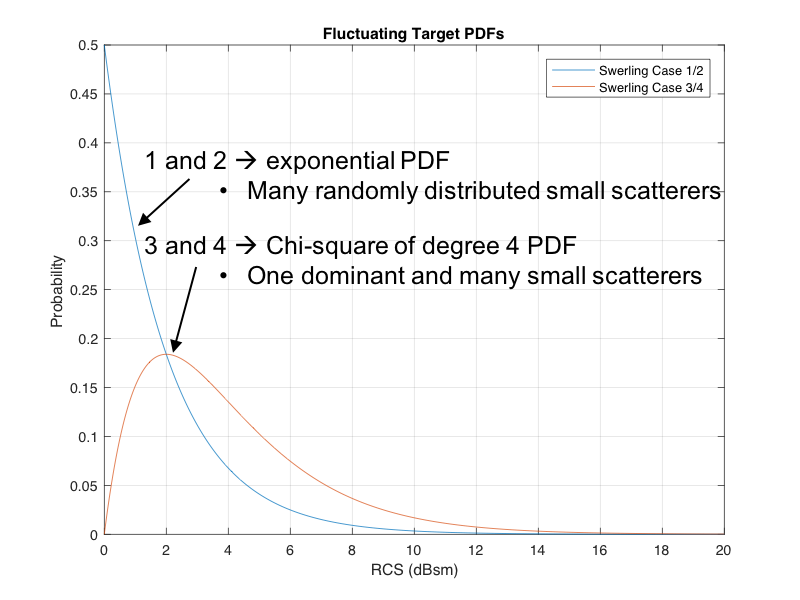
\includegraphics[width=4in]{../media/multistatic/swerling_pdfs.png}
  \end{center}
  \renewcommand{\baselinestretch}{1} \small\normalsize
  \begin{quote}
    \caption[Swerling Target Fluctuation Model PDFs]{Swerling Target Fluctuation Model PDFs\label{env_fig:2}}
  \end{quote}
\end{figure}
\renewcommand{\baselinestretch}{2} \small\normalsize

The long decorrelation time covers the case where the target RCS can be considered constant over the time the RADAR performs a single scan and the short decorrelation time covers the case where the target RCS changes on a pulse to pulse basis. Modern RADAR systems operate in frequency agile modes where the carrier frequency is changed each pulse, in which case the decorrelation time can be considered to be short. A fluctuating signal can have a significant effect on the $P_d$, as seen in Figure \ref{env_fig:3} which shows $P_d$ as a function of SNR for the nonfluctating case and each of the $4$ Swerling cases. In this figure, we can see that using the wrong PDF can result in significantly overestimating the $P_d$.
\begin{figure}[H]
  \begin{center}
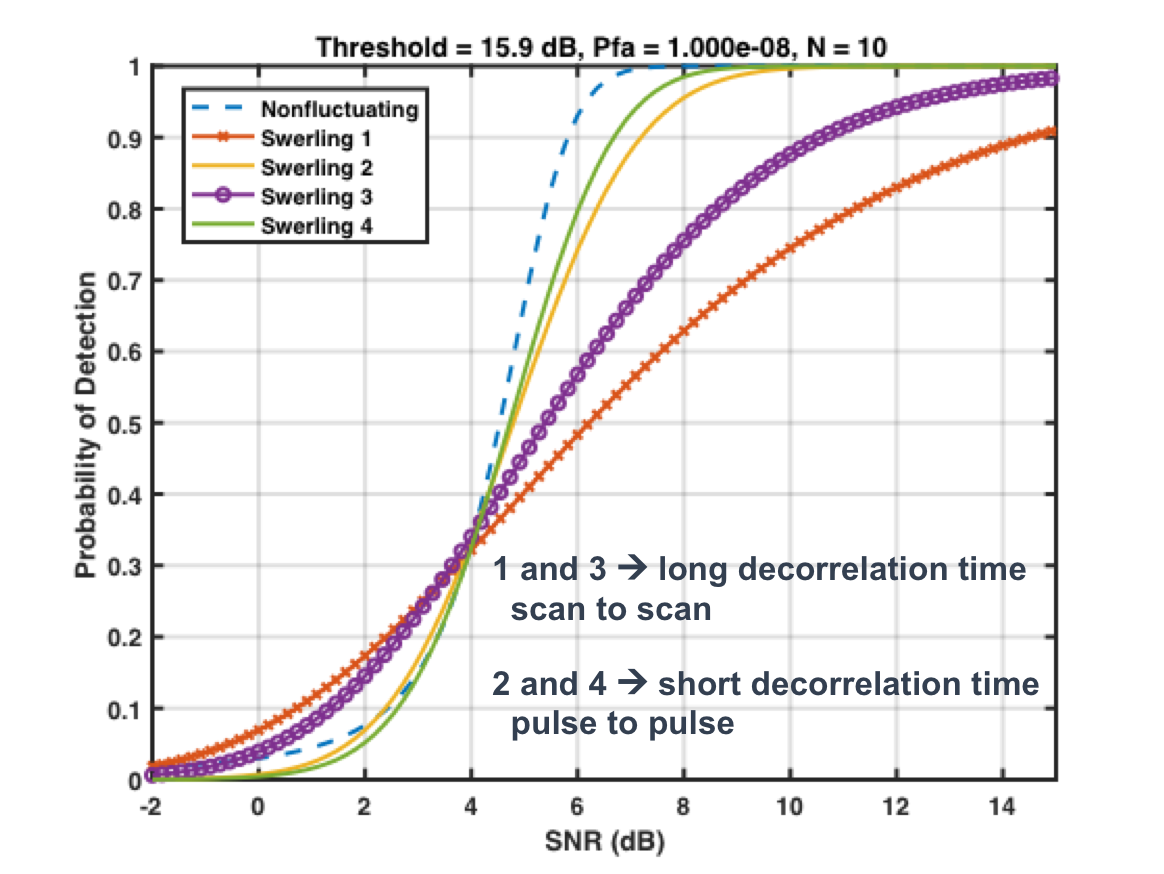
\includegraphics[width=4in]{../media/multistatic/swerling_pd.png}
  \end{center}
  \renewcommand{\baselinestretch}{1} \small\normalsize
  \begin{quote}
    \caption[Swerling Target Fluctuation Model Probability of Detection]{Swerling Target Fluctuation Model Probability of Detection\label{env_fig:3}}
  \end{quote}
\end{figure}
\renewcommand{\baselinestretch}{2} \small\normalsize

Figure \ref{env_fig:3} also shows that the $P_d$ is higher with a dominant scatterer than with a collection of uniform scatterers and that it is higher for a short decorrelation time than a long decorrelation time. We can force the decorrelation time to be short by operating in a frequency agile mode, but we generally have no control over the target configuration.

Modeling the RCS for a Swerling fluctuating target is straightforward. We can generate random variables following a Chi-squared distribution of degree $n$ by the sum of $n$ squared normally distributed random variables with zero mean and unit variance. The mean of the Chi-squared distribution is equal to the degree, so to force the mean to the deterministic value, we need to add this value and subtract the degree.

Swerling cases 1 and 2 follow a Chi-squared distribution of degree 2. To generate a random variable, $w_{1,2}$, for our RCS, we need to generate 2 normally distributed random variables, $u_1$ and $u_2$. Then, $w_{1,2}$ is given by Equation \ref{env_eq:8}, where $\sigma$ is the deterministic RCS value.
\begin{equation}
  \label{env_eq:8}
w_{1,2} = u_1^2 + u_2^2 + \sigma - 2
  \end{equation}

Swerling cases 3 and 4 follow a Chi-squared distribution of degree 4. To generate a random variable, $w_{3,4}$, for our RCS, we need to generate 4 normally distributed random variables, $u_1$, $u_2$, $u_3$, and $u_4$. Then, $w_{3,4}$ is given by Equation \ref{env_eq:9}, where $\sigma$ is again the deterministic RCS value.
\begin{equation}
  \label{env_eq:9}
w_{3,4} = u_1^2 + u_2^2 + u_3^2 + u_4^2 + \sigma - 4
  \end{equation}
  
The decorrelation time then determines when to perform the random draws; this can be every pulse, every CPI, or at some predetermined time interval. When we have multiple transmitters, we need to be careful about when to schedule the random draws so that one actor does not influence the other.  